\section*{Ubicación de sensores PT100 Y NTC}

Para la ubicación de los sensores RTD se considero primero la implementación de la planta térmica mostrada en la figura \ref{fig:planta-termica} la cual cuenta con el disipador aislado y en el cual se colocaron ambos sensores térmicos.

\begin{figure}[h]
	\centering
	
\includegraphics[width=0.6\linewidth]{media/planta-termica}
	\caption{Planta termica y ubicación de los sensores}
	\label{fig:planta-termica}
\end{figure}

\section*{Incremento de temperatura de T hasta 40°C}

Para el incremento de temperatura, este proceso se automatizo para incrementarse en $1.5C°$ después de que el sistema de control de temperatura haya alcanzando el punto de estabilidad considerando para el experimento un rango de temperaturas desde $22C°$ hasta los $41.5C°$, en la figura \ref{fig:graphics-incremento-temperatura} se puede apreciar la automatización de este proceso de forma visual mediante el cambio de la temperatura en forma constante.

% TODO: \usepackage{graphicx} required
\begin{figure}[h]
	\centering
	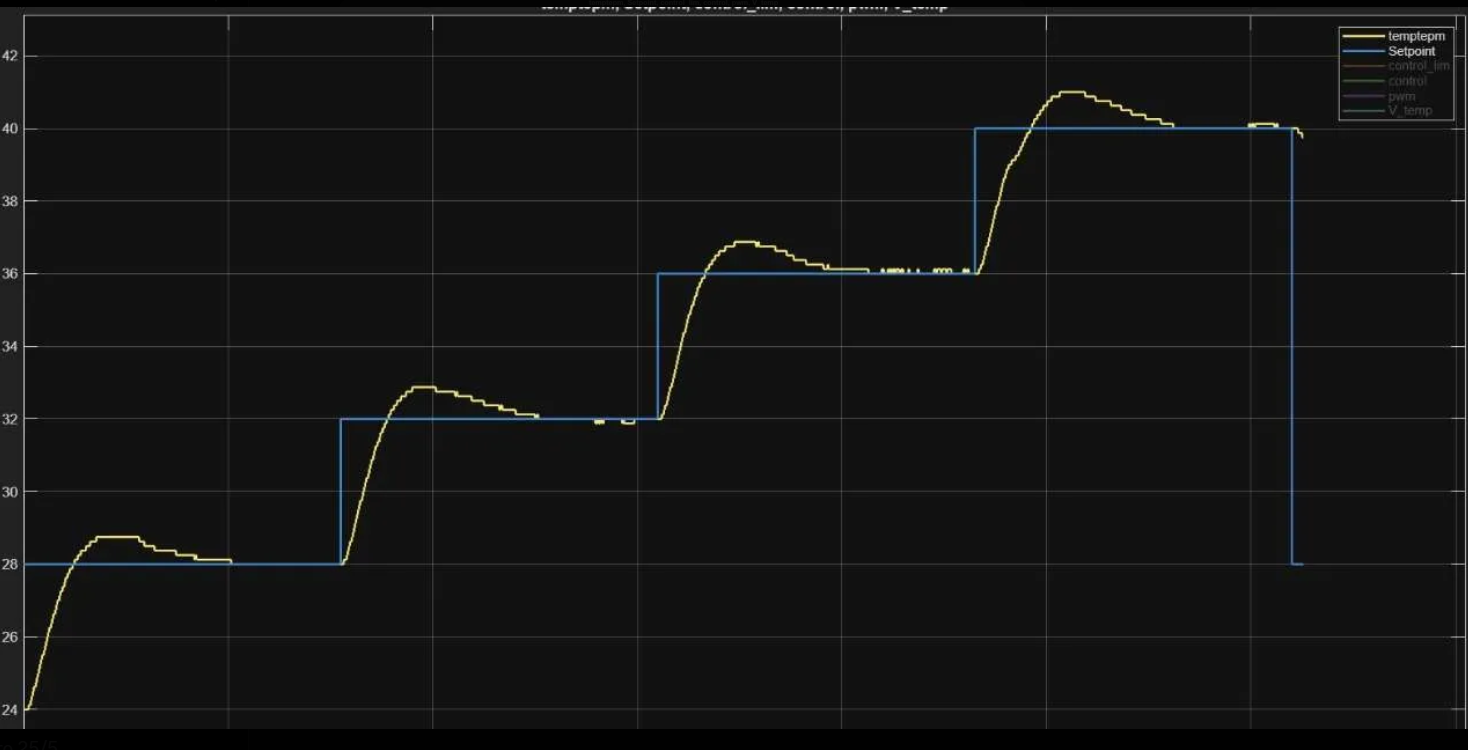
\includegraphics[width=0.7\linewidth]{media/graphics-incremento-temperatura}
	\caption{Incremento de temperatura}
	\label{fig:graphics-incremento-temperatura}
\end{figure}


\section*{Curva de tensión y resistencia calculada del PT100}

Con el control de temperatura establecido y definida la ganancia del circuito en función a la resistencia variable en función a la temperatura de los RTD es posible determinar el valor de esta ultima al conocer la corriente que circula por las resistencias de entrada en cada amplificador y el voltaje de salida o en función a la ganancia definida entre el voltaje de entrada y el voltaje medido en la salida usándose el segundo método durante la experimentación con la finalidad de validar un método diferente al propuesto.

Siendo así que en las figuras \ref{fig:tension-temp-pt100} y \ref{fig:tension-res-pt100} se puede apreciar las diferentes curvas de tensión, resistencias vs temperatura para los RTD propuestos

% TODO: \usepackage{graphicx} required
\begin{figure}[h]
	\centering
	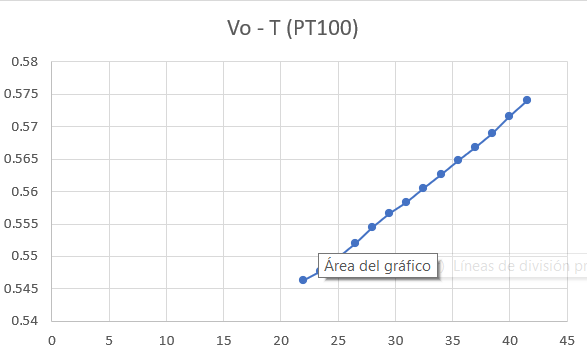
\includegraphics[width=0.7\linewidth]{media/tension-temp-pt100}
	\caption{Curva de tensión vs temperatura - PT100}
	\label{fig:tension-temp-pt100}
\end{figure}

% TODO: \usepackage{graphicx} required
\begin{figure}[h]
	\centering
	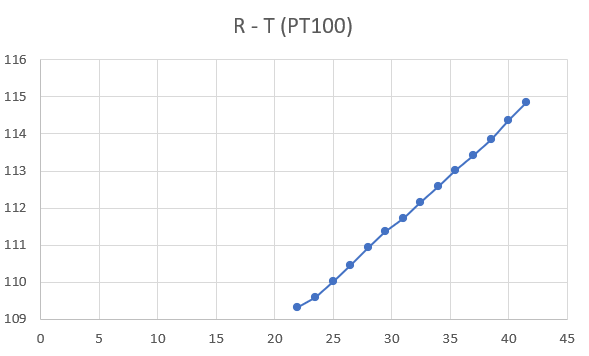
\includegraphics[width=0.7\linewidth]{media/tension-res-pt100}
	\caption{Curva de resistencia vs temperatura -PT100}
	\label{fig:tension-res-pt100}
\end{figure}

Destacando así que las curvas se asemejan a las curvas experimentales y el comportamiento descrito por los fabricantes para el rango de temperatura previamente mencionado.

\section*{Curva de tensión y resistencia para el NTC}

En las figuras \ref{fig:tension-temp-pt100} y \ref{fig:tension-res-ntc} se muestran las curvas para el NTC descrita por un exponencial decreciente debido a que este tipo de sensor disminuye su resistencia interna conforme aumenta su temperatura.

% TODO: \usepackage{graphicx} required
\begin{figure}[h]
	\centering
	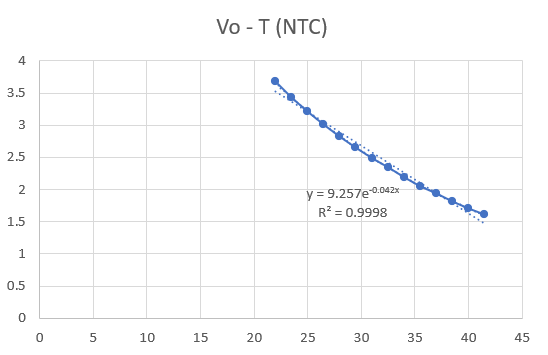
\includegraphics[width=0.7\linewidth]{media/tension-temp-NTC}
	\caption{Curva de tensión vs temperatura NTC}
	\label{fig:tension-temp-ntc}
\end{figure}

% TODO: \usepackage{graphicx} required
\begin{figure}[h]
	\centering
	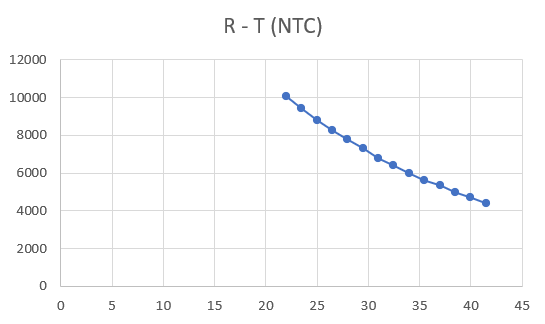
\includegraphics[width=0.7\linewidth]{media/tension-res-NTC}
	\caption{Curva de tensión vs resistencia - NTC}
	\label{fig:tension-res-ntc}
\end{figure}

\section*{Pendiente de resistencia vs temperatura PT100 cuando el valor es de 0.385 $\Omega /C°$}

A partir de la gráfica mostrada en la figura \ref{fig:tension-res-pt100} la línea de tendencia para los datos obtenidos aplicando una regresión lineal simple se describe en \ref{eq:recta-res-pt100}

\begin{equation}
	R(T) = 0.2845T + 102.94
	\label{eq:recta-res-pt100}
\end{equation}

Y de la cual se puede obtener el valor de la pendiente respecto a la resistencia al derivar la expresión \ref{eq:recta-res-pt100} respecto a la temperatura obteniendo una variación por grado $°C$ de $0.2845$ y que a nivel de gráfico. 

\section*{Curva de resistencia temperatura NTC y la expresión exponencial decreciente}

La curva de resistencia vs temperatura se aprecia en la figura \ref{fig:tension-res-ntc} con las características asociadas a la ecuación \ref{eq:res-temp-ntc}

\begin{equation}
	R(T) = 25375e^{-0.042T}
	\label{eq:res-temp-ntc}
\end{equation}

Esta luego de realizar el ajuste de la curva mediante regresión exponencial para ajustar los datos experimentales a un modelo matemático, obteniendo así para este modelo obtenido para el NTC a los 25$C°$ 8.799K$\Omega$ según los datos medidos y de 8.908K $C°$ para el modelo generado.

Sin embargo como método adicional debido a características propias del NTC es posible realizar una calibración al considerar el logaritmo de la resistencia respecto a la inversa de la temperatura expresada en Kelvin y mostrada en la figura \ref{fig:linealizacion-curva-ntc} y como se describe en \cite{Guemez2003CalibracionTermistor}

% TODO: \usepackage{graphicx} required
\begin{figure}[h]
	\centering
	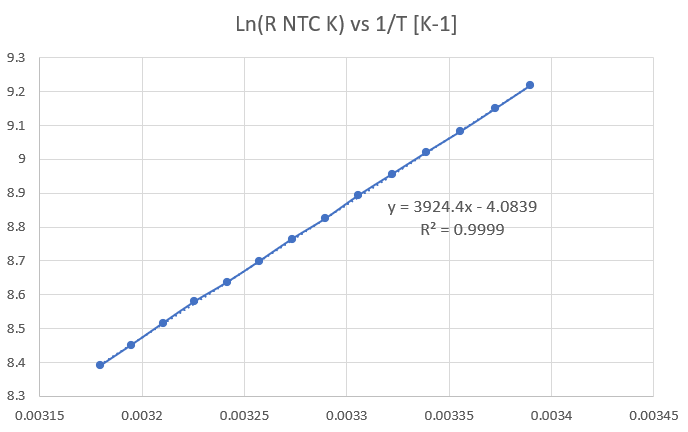
\includegraphics[width=0.7\linewidth]{media/linealizacion-curva-NTC}
	\caption{Linealización de la curva exponencial LN(R NTC [K]) vs 1/T [K-1]}
	\label{fig:linealizacion-curva-ntc}
\end{figure}

Y la cual se puede usar para representar le ecuación \ref{eq:ntc} del NTC 

\begin{equation}
	T(C) = \frac{B}{ln(R NTC K) + C} - 27395
	\label{eq:ntc}
\end{equation}

Obteniendo los factores B y C mediante regresión lineal aplicada en la figura \ref{fig:linealizacion-curva-ntc} se obtiene la siguiente ecuación de la recta \ref{eq:recta-ntc-linealizada}

\begin{equation}
	y = 3924.4x - 4.0839
	\label{eq:recta-ntc-linealizada}
\end{equation}

De donde se obtiene que $B = 3924.4$ y $C = -4.0839$ obteniendo finalmente la expresión modificada a partir de \ref{eq:ntc} con los valores obtenidos

\begin{equation}
	T(C) = \frac{3924.4}{ln(R NTC K) - 4.0839} - 27395
\end{equation}
